\documentclass[aspectratio=169,10pt]{beamer}
\usetheme{Madrid}

\usepackage[T1]{fontenc}
\usepackage{lmodern}
\usepackage{booktabs,array}
\usepackage{tikz}
\usetikzlibrary{positioning,arrows.meta,shapes.geometric,shapes.misc,fit,backgrounds,calc}

\definecolor{kfcblue}{HTML}{185FA5}
\definecolor{kfcteal}{HTML}{0F6E56}
\definecolor{kfcpurple}{HTML}{534AB7}
\definecolor{kfcgray}{HTML}{5F5E5A}
\definecolor{lightblue}{HTML}{E6F1FB}
\definecolor{lightteal}{HTML}{E1F5EE}
\definecolor{lightpurple}{HTML}{EEEDFE}
\definecolor{lightgray}{HTML}{F1EFE8}
\definecolor{lightamber}{HTML}{FAEEDA}

\setbeamertemplate{navigation symbols}{}
\renewcommand{\arraystretch}{1.25}
\newcommand{\ep}[1]{\texttt{\small #1}}

\title{GameTrend Radar}
\subtitle{Real-time trend analytics for Roblox and Steam games\\Project Milestone 2: data acquisition and pre-processing}
\author[Team KFC]{Bart\l{}omiej Borycki \and Micha\l{} Iwaniuk \and Jan Cwalina \and Mi\l{}osz Choda\'n}
\institute[]{Team KFC}
\date{}

\begin{document}

%----------------------------------------------------------------------
\begin{frame}
  \titlepage
\end{frame}

%----------------------------------------------------------------------
\begin{frame}{Problem and users}
  \begin{itemize}
    \item Roblox is driven by short trends; many mechanics come from Steam hits.
    \item Users: Roblox developers, small studios, game-market analysts.
    \item They ask three questions:
    \begin{itemize}
      \item What is rising right now?
      \item Where did the trend come from?
      \item How crowded is the niche?
    \end{itemize}
    \item We answer them with live player data from Roblox and Steam, a lambda pipeline and a dashboard.
  \end{itemize}
\end{frame}

%----------------------------------------------------------------------
\begin{frame}{Core use case}
  \centering
  \resizebox{0.92\linewidth}{!}{% BPMN: monitor a trending Roblox game and trace its possible Steam origin.
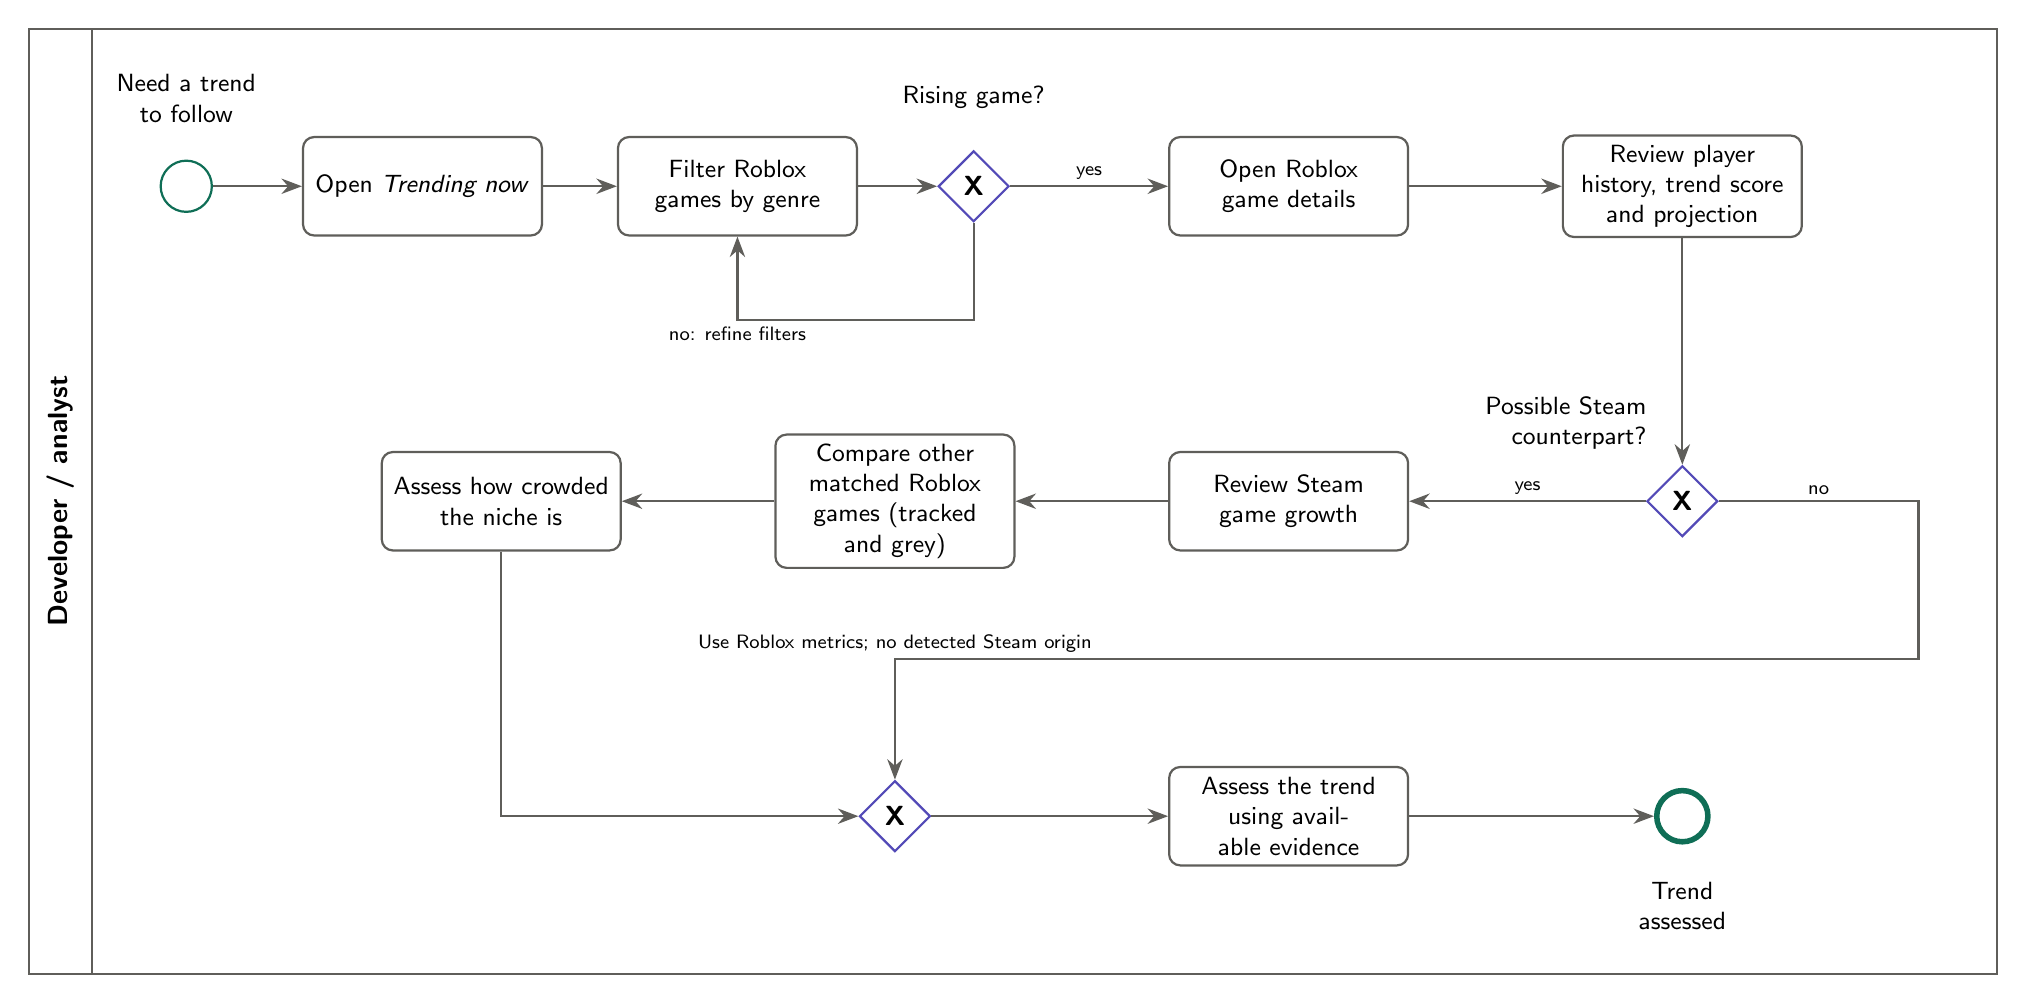
\begin{tikzpicture}[
  font=\sffamily\small,
  task/.style={rectangle, rounded corners=4pt, draw=kfcgray, fill=white, thick, minimum height=1.25cm, align=center, text width=2.8cm},
  start/.style={circle, draw=kfcteal, thick, minimum size=0.65cm, fill=white},
  endev/.style={circle, draw=kfcteal, line width=2pt, minimum size=0.65cm, fill=white},
  gw/.style={diamond, draw=kfcpurple, thick, fill=white, minimum size=0.9cm, inner sep=0pt, font=\sffamily\bfseries},
  flow/.style={-{Stealth[length=2.6mm]}, thick, draw=kfcgray},
  lbl/.style={font=\sffamily\scriptsize, fill=white, inner sep=2pt}
]
\draw[thick, kfcgray] (0,0) rectangle (25,-12);
\draw[thick, kfcgray] (0.8,0) -- (0.8,-12);
\node[rotate=90, font=\sffamily\bfseries] at (0.4,-6) {Developer / analyst};

\node[start] (start) at (2,-2) {};
\node[above=0.35cm of start, align=center] {Need a trend\\to follow};
\node[task] (browse) at (5,-2) {Open \emph{Trending now}};
\node[task] (filter) at (9,-2) {Filter Roblox games by genre};
\node[gw] (rising) at (12,-2) {X};
\node[above=0.4cm of rising] {Rising game?};
\node[task] (details) at (16,-2) {Open Roblox game details};
\node[task] (metrics) at (21,-2) {Review player history, trend score and projection};

\node[gw] (linked) at (21,-6) {X};
\node[above left=0.3cm and 0.1cm of linked, align=right] {Possible Steam\\counterpart?};
\node[task] (steam) at (16,-6) {Review Steam game growth};
\node[task] (others) at (11,-6) {Compare other matched Roblox games (tracked and grey)};
\node[task] (niche) at (6,-6) {Assess how crowded the niche is};
\node[gw] (merge) at (11,-10) {X};
\node[task] (assess) at (16,-10) {Assess the trend using available evidence};
\node[endev] (end) at (21,-10) {};
\node[below=0.35cm of end, align=center] {Trend\\assessed};

\draw[flow] (start) -- (browse);
\draw[flow] (browse) -- (filter);
\draw[flow] (filter) -- (rising);
\draw[flow] (rising) -- node[lbl, above]{yes} (details);
\draw[flow] (rising.south) -- (12,-3.7) -| node[lbl, pos=0.5, below]{no: refine filters} (filter.south);
\draw[flow] (details) -- (metrics);
\draw[flow] (metrics) -- (linked);
\draw[flow] (linked) -- node[lbl, above]{yes} (steam);
\draw[flow] (steam) -- (others);
\draw[flow] (others) -- (niche);
\draw[flow] (niche.south) |- (merge.west);
\draw[flow] (linked.east) -- node[lbl, above]{no} (24,-6) -- (24,-8) -| node[lbl, pos=0.5, above]{Use Roblox metrics; no detected Steam origin} (merge.north);
\draw[flow] (merge) -- (assess);
\draw[flow] (assess) -- (end);
\end{tikzpicture}
}
  \vspace{2mm}

  \small Monitor trending Roblox games and trace their possible Steam origin.
\end{frame}

%----------------------------------------------------------------------
\begin{frame}{Changes since Milestone 1}
  \centering
  \begin{tabular}{>{\bfseries}l l l}
    \toprule
    Topic & Milestone 1 & Milestone 2\\
    \midrule
    Core use case & Steam $\rightarrow$ Roblox opportunities & trending Roblox games\\
    Data source & live APIs & recorded archive + mock API\\
    Polling & every 5--15 min & every source $\le$ 15 s\\
    Model training & every hour & once, on a fixed slice\\
    \bottomrule
  \end{tabular}

  \vspace{5mm}
  \small Main reason: the live APIs are rate-limited, so we record once and replay.
\end{frame}

%----------------------------------------------------------------------
\begin{frame}{Conceptual data model}
  \centering
  \resizebox{!}{0.82\textheight}{% Conceptual data model: entities and relationships with cardinalities.
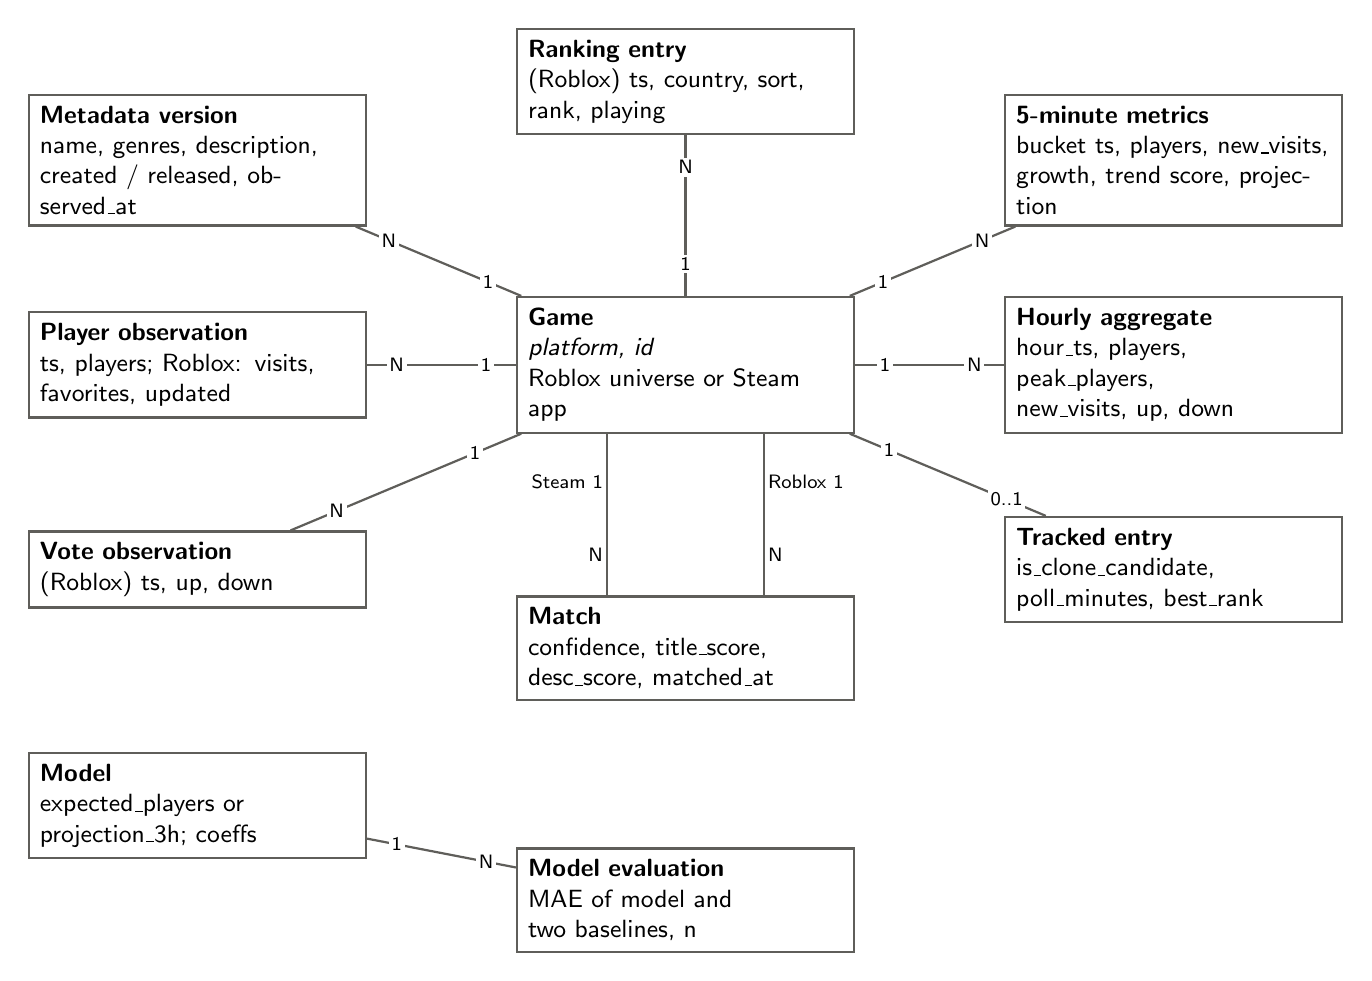
\begin{tikzpicture}[
  font=\sffamily\small,
  ent/.style={rectangle, draw=kfcgray, thick, fill=white, align=left, text width=4.0cm, inner sep=4pt},
  rel/.style={thick, draw=kfcgray},
  card/.style={font=\sffamily\scriptsize, fill=white, inner sep=1pt}
]
\node[ent] (game) at (0,0) {\textbf{Game}\\\textit{platform, id}\\Roblox universe or Steam app};
\node[ent] (meta) at (-6.2,2.6) {\textbf{Metadata version}\\name, genres, description,\\created / released, observed\_at};
\node[ent] (obs) at (-6.2,0) {\textbf{Player observation}\\ts, players; Roblox: visits,\\favorites, updated};
\node[ent] (votes) at (-6.2,-2.6) {\textbf{Vote observation}\\(Roblox) ts, up, down};
\node[ent] (sort) at (0,3.6) {\textbf{Ranking entry}\\(Roblox) ts, country, sort,\\rank, playing};
\node[ent] (m5) at (6.2,2.6) {\textbf{5-minute metrics}\\bucket ts, players, new\_visits,\\growth, trend score, projection};
\node[ent] (mh) at (6.2,0) {\textbf{Hourly aggregate}\\hour\_ts, players, peak\_players,\\new\_visits, up, down};
\node[ent] (match) at (0,-3.6) {\textbf{Match}\\confidence, title\_score,\\desc\_score, matched\_at};
\node[ent] (track) at (6.2,-2.6) {\textbf{Tracked entry}\\is\_clone\_candidate,\\poll\_minutes, best\_rank};
\node[ent] (model) at (-6.2,-5.6) {\textbf{Model}\\expected\_players or\\projection\_3h; coeffs};
\node[ent] (eval) at (0,-6.8) {\textbf{Model evaluation}\\MAE of model and\\two baselines, n};

\draw[rel] (game) -- node[card, pos=0.2]{1} node[card, pos=0.8]{N} (meta);
\draw[rel] (game) -- node[card, pos=0.2]{1} node[card, pos=0.8]{N} (obs);
\draw[rel] (game) -- node[card, pos=0.2]{1} node[card, pos=0.8]{N} (votes);
\draw[rel] (game) -- node[card, pos=0.2]{1} node[card, pos=0.8]{N} (sort);
\draw[rel] (game) -- node[card, pos=0.2]{1} node[card, pos=0.8]{N} (m5);
\draw[rel] (game) -- node[card, pos=0.2]{1} node[card, pos=0.8]{N} (mh);
\draw[rel] (game) -- node[card, pos=0.2]{1} node[card, pos=0.8]{0..1} (track);
\draw[rel] ([xshift=-1.0cm]game.south) -- node[card, pos=0.3, left]{Steam 1} node[card, pos=0.75, left]{N} ([xshift=-1.0cm]match.north);
\draw[rel] ([xshift=1.0cm]game.south) -- node[card, pos=0.3, right]{Roblox 1} node[card, pos=0.75, right]{N} ([xshift=1.0cm]match.north);
\draw[rel] (model) -- node[card, pos=0.2]{1} node[card, pos=0.8]{N} (eval);
\end{tikzpicture}
}
\end{frame}

%----------------------------------------------------------------------
\begin{frame}{Data sets}
  \centering
  \begin{tabular}{>{\bfseries}l l l}
    \toprule
    Feed & Content & Inflow\\
    \midrule
    Roblox games & players, visits, updates & every $\sim$100 s\\
    Roblox votes & likes, dislikes & every 5 min\\
    Roblox rankings & position per country & every 15 min\\
    Steam players & players & every 5 min\\
    Steam details & genre, release, description & once per game\\
    \bottomrule
  \end{tabular}

  \vspace{5mm}
  \begin{itemize}
    \item 6 days recorded (5--11 Nov 2026), JSON, $\sim$2.3M records/day.
    \item 1,641 Roblox games with full player history.
  \end{itemize}
\end{frame}

%----------------------------------------------------------------------
\begin{frame}{Data quality}
  \centering
  \begin{tabular}{>{\bfseries}l l}
    \toprule
    Issue & Handling\\
    \midrule
    API errors ($<$0.1\%) & retry with back-off\\
    $\sim$2 h recording gap & metric left absent\\
    Steam game without stats & no event, never 0\\
    Search hit not tracked (79\%) & title-only match, shown in grey\\
    Duplicates after replays & dropped by readers\\
    \bottomrule
  \end{tabular}

  \vspace{5mm}
  \small Rule everywhere: a missing value is absent, never zero.
\end{frame}

%----------------------------------------------------------------------
\begin{frame}{Data acquisition}
  \centering
  \resizebox{\linewidth}{!}{%
  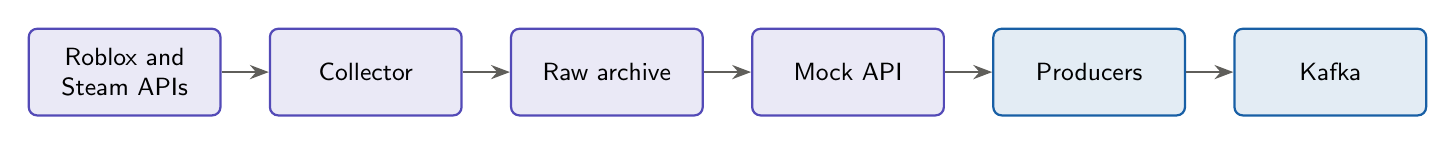
\begin{tikzpicture}[font=\sffamily\small,
    box/.style={rectangle, rounded corners=3pt, thick, align=center, minimum height=1.1cm, text width=2.2cm},
    tool/.style={box, draw=kfcpurple, fill=kfcpurple!12},
    ing/.style={box, draw=kfcblue, fill=kfcblue!12},
    arr/.style={-{Stealth[length=2.4mm]}, thick, draw=kfcgray}]
    \node[tool] (api) {Roblox and Steam APIs};
    \node[tool, right=0.6cm of api] (col) {Collector};
    \node[tool, right=0.6cm of col] (arc) {Raw archive};
    \node[tool, right=0.6cm of arc] (mock) {Mock API};
    \node[ing, right=0.6cm of mock] (prod) {Producers};
    \node[ing, right=0.6cm of prod] (kafka) {Kafka};
    \draw[arr] (api) -- (col); \draw[arr] (col) -- (arc); \draw[arr] (arc) -- (mock);
    \draw[arr] (mock) -- (prod); \draw[arr] (prod) -- (kafka);
  \end{tikzpicture}}

  \vspace{6mm}
  \begin{itemize}
    \item Collector saves every API response unchanged, with its original time.
    \item Mock API replays the archive like the real APIs, also faster.
    \item Producers validate events and send them to Kafka; same code for mock and live.
    \item Roblox limits us to about one request per 3 s.
  \end{itemize}
\end{frame}

%----------------------------------------------------------------------
\begin{frame}{Lambda architecture}
  \centering
  \resizebox{\linewidth}{!}{% Solution architecture (lambda). Implemented: solid border, tinted fill. Planned (next phases): dashed border, white fill, PLANNED tag.
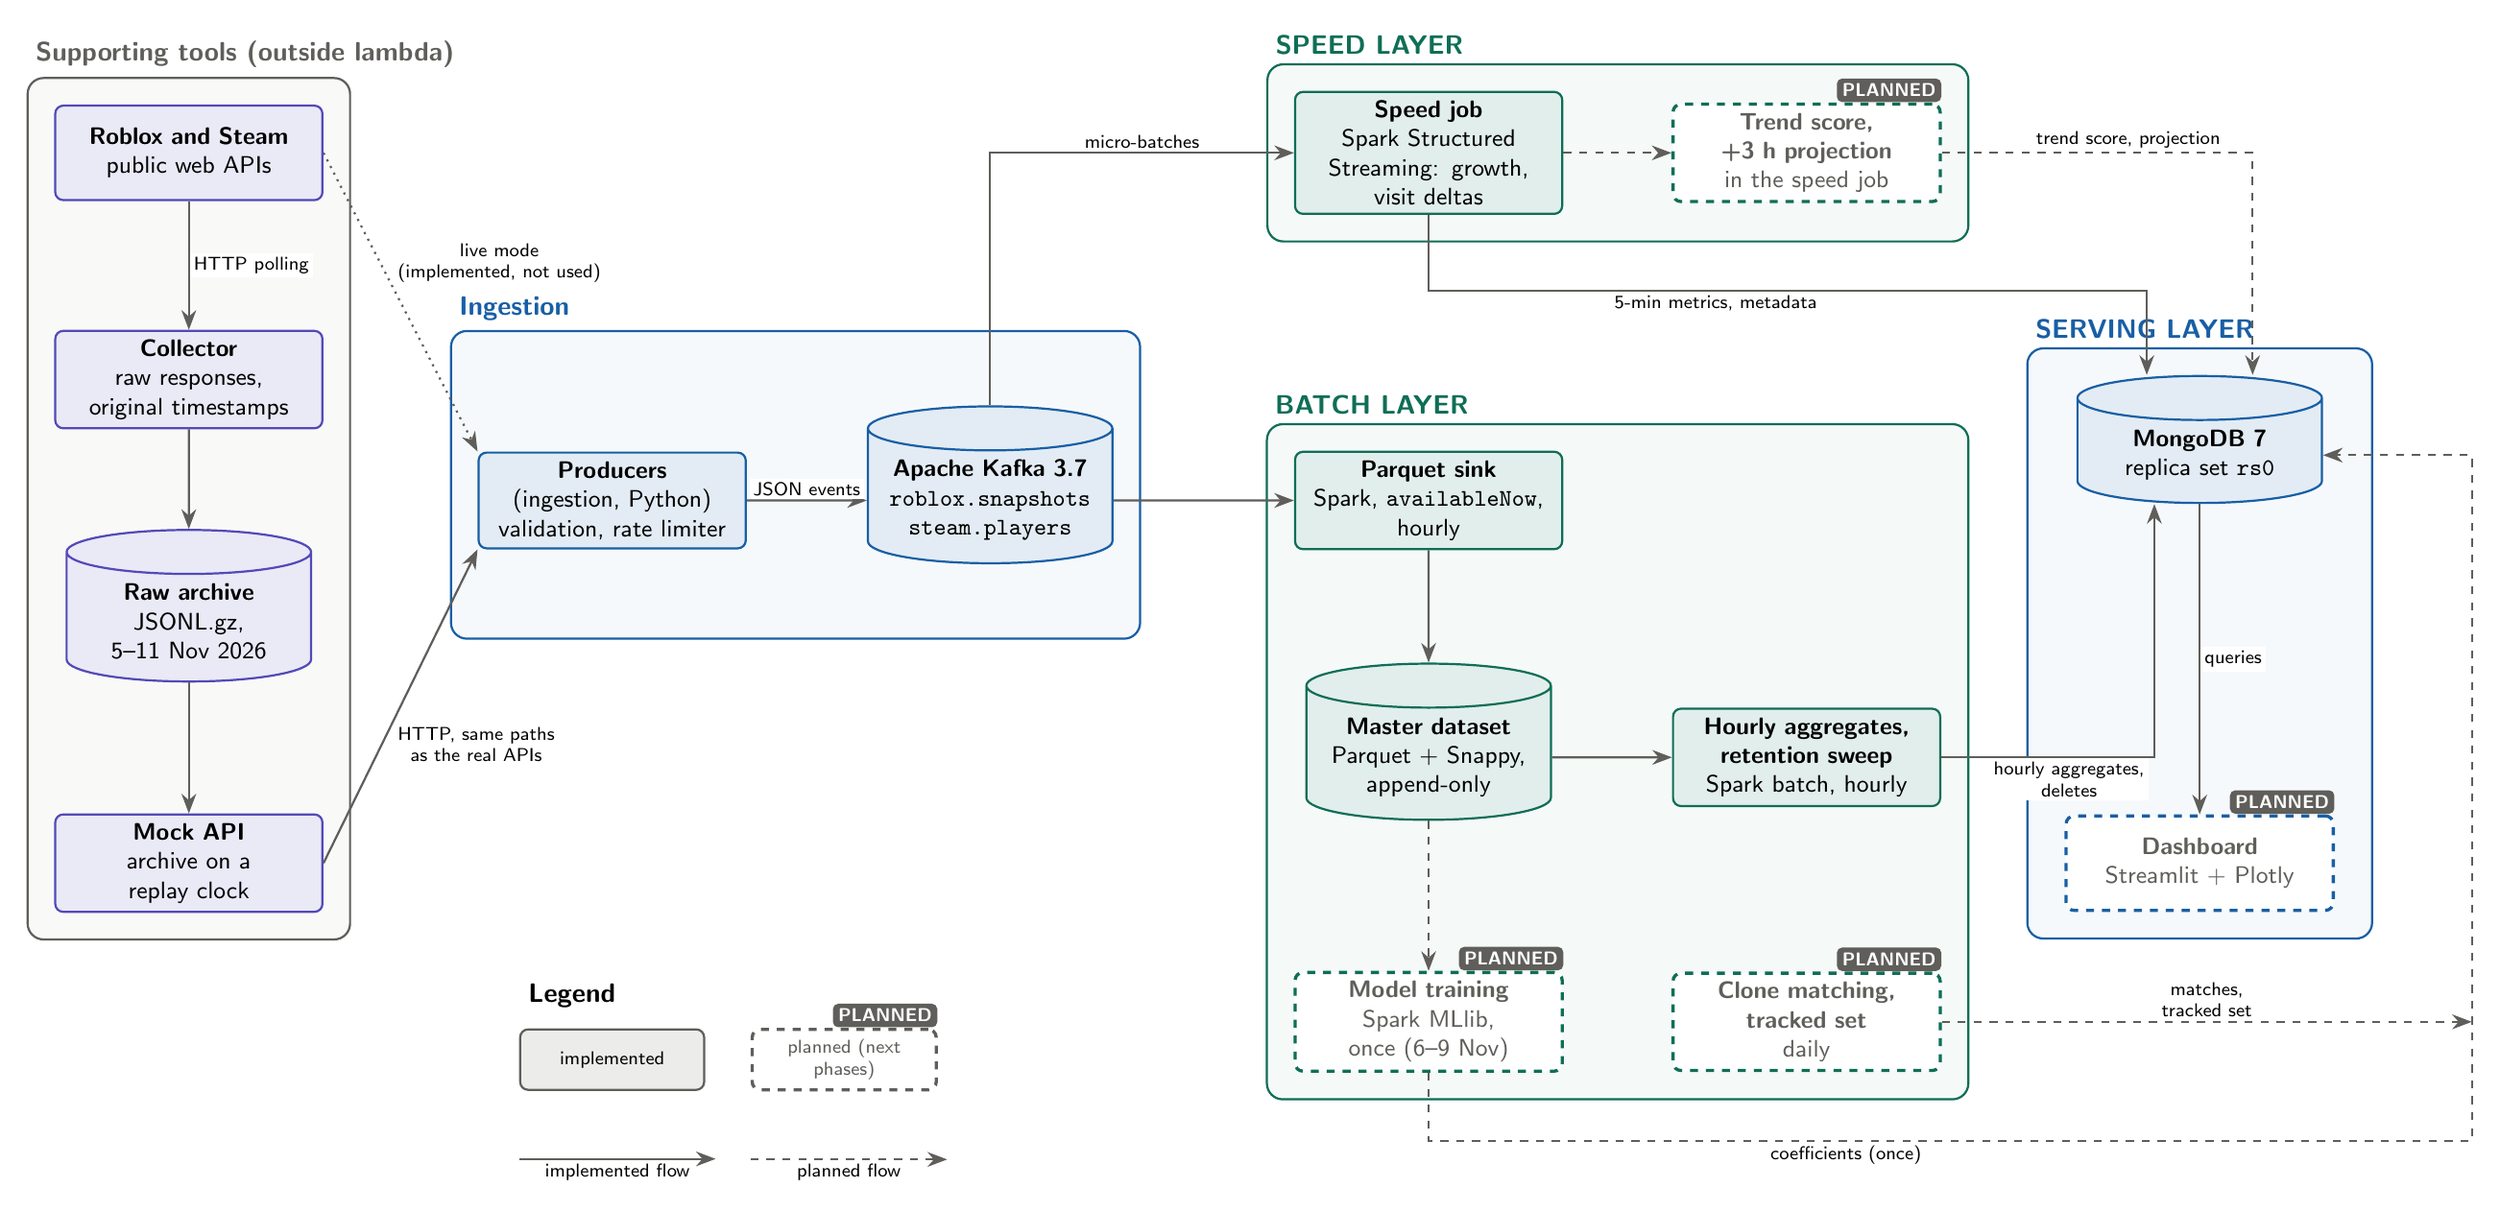
\begin{tikzpicture}[
  font=\sffamily\small,
  box/.style={rectangle, rounded corners=3pt, draw=#1, fill=#1!12, thick, align=center, minimum height=1.25cm, text width=3.3cm},
  box/.default=kfcgray,
  db/.style={cylinder, shape border rotate=90, aspect=0.18, draw=#1, fill=#1!12, thick, align=center, minimum height=1.45cm, text width=3.0cm},
  db/.default=kfcgray,
  plan/.style={dashed, fill=white, text=kfcgray, line width=1.2pt},
  tag/.style={font=\sffamily\scriptsize\bfseries, text=white, fill=kfcgray, rounded corners=2pt, inner sep=2pt, anchor=south east},
  arr/.style={-{Stealth[length=2.6mm]}, thick, draw=kfcgray},
  parr/.style={arr, dashed},
  altarr/.style={arr, dotted},
  lab/.style={font=\sffamily\scriptsize, fill=white, inner sep=1.5pt, align=center},
  layer/.style={rectangle, rounded corners=6pt, draw=#1, fill=#1!4, thick, inner sep=10pt},
  ltitle/.style={font=\sffamily\bfseries, text=#1, anchor=south west}
]
% ---------------- sources and supporting tools
\node[box=kfcpurple] (api) at (0,4.6) {\textbf{Roblox and Steam}\\public web APIs};
\node[box=kfcpurple] (coll) at (0,1.6) {\textbf{Collector}\\raw responses,\\original timestamps};
\node[db=kfcpurple] (raw) at (0,-1.6) {\textbf{Raw archive}\\JSONL.gz,\\5--11 Nov 2026};
\node[box=kfcpurple] (mock) at (0,-4.8) {\textbf{Mock API}\\archive on a\\replay clock};
% ---------------- ingestion
\node[box=kfcblue] (prod) at (5.6,0) {\textbf{Producers}\\(ingestion, Python)\\validation, rate limiter};
\node[db=kfcblue] (kafka) at (10.6,0) {\textbf{Apache Kafka 3.7}\\\texttt{roblox.snapshots}\\\texttt{steam.players}};
% ---------------- speed layer
\node[box=kfcteal] (speed) at (16.4,4.6) {\textbf{Speed job}\\Spark Structured\\Streaming: growth,\\visit deltas};
\node[box=kfcteal, plan] (score) at (21.4,4.6) {\textbf{Trend score,}\\\textbf{+3 h projection}\\in the speed job};
% ---------------- batch layer
\node[box=kfcteal] (sink) at (16.4,0) {\textbf{Parquet sink}\\Spark, \texttt{availableNow},\\hourly};
\node[db=kfcteal] (master) at (16.4,-3.4) {\textbf{Master dataset}\\Parquet + Snappy,\\append-only};
\node[box=kfcteal] (agg) at (21.4,-3.4) {\textbf{Hourly aggregates,}\\\textbf{retention sweep}\\Spark batch, hourly};
\node[box=kfcteal, plan] (train) at (16.4,-6.9) {\textbf{Model training}\\Spark MLlib,\\once (6--9 Nov)};
\node[box=kfcteal, plan] (match) at (21.4,-6.9) {\textbf{Clone matching,}\\\textbf{tracked set}\\daily};
% ---------------- serving layer
\node[db=kfcblue] (mongo) at (26.6,0.6) {\textbf{MongoDB 7}\\replica set \texttt{rs0}};
\node[box=kfcblue, plan] (dash) at (26.6,-4.8) {\textbf{Dashboard}\\Streamlit + Plotly};

% PLANNED tags
\foreach \n in {score, train, match, dash} {\node[tag] at (\n.north east) {PLANNED};}

% ---------------- layers
\begin{scope}[on background layer]
  \node[layer=kfcgray, fit=(api)(coll)(raw)(mock), label={[ltitle=kfcgray]north west:Supporting tools (outside lambda)}] {};
  \node[layer=kfcblue, fit=(prod)(kafka), inner ysep=28pt, label={[ltitle=kfcblue]north west:Ingestion}] {};
  \node[layer=kfcteal, fit=(speed)(score), label={[ltitle=kfcteal]north west:SPEED LAYER}] {};
  \node[layer=kfcteal, fit=(sink)(master)(agg)(train)(match), label={[ltitle=kfcteal]north west:BATCH LAYER}] {};
  \node[layer=kfcblue, fit=(mongo)(dash), inner xsep=14pt, label={[ltitle=kfcblue]north west:SERVING LAYER}] {};
\end{scope}

% ---------------- flows
\draw[arr] (api) -- node[lab, right]{HTTP polling} (coll);
\draw[arr] (coll) -- (raw);
\draw[arr] (raw) -- (mock);
\draw[arr] (mock.east) -- node[lab, pos=0.45, below right]{HTTP, same paths\\as the real APIs} (prod.south west);
\draw[altarr] (api.east) -- node[lab, pos=0.45, above right]{live mode\\(implemented, not used)} (prod.north west);
\draw[arr] (prod) -- node[lab, above]{JSON events} (kafka);
\draw[arr] (kafka.north) |- node[lab, pos=0.75, above]{micro-batches} (speed.west);
\draw[arr] (kafka.east) -- (sink.west);
\draw[parr] (speed) -- (score);
\draw[arr] (sink) -- (master);
\draw[arr] (master) -- (agg);
\draw[parr] (master) -- (train);
\draw[arr] (speed.south) |- ++(0,-1.0) -| node[lab, pos=0.2, below]{5-min metrics, metadata} ([xshift=-0.7cm]mongo.north);
\draw[parr] (score.east) -| node[lab, pos=0.3, above]{trend score, projection} ([xshift=0.7cm]mongo.north);
\draw[arr] (agg.east) -| node[lab, pos=0.3, below]{hourly aggregates,\\deletes} ([xshift=-0.6cm]mongo.south);
\draw[parr] (train.south) -- ++(0,-0.9) -| node[lab, pos=0.2, below]{coefficients (once)} (30.2,-1) |- (mongo.east);
\draw[parr] (match.east) -- node[lab, above]{matches,\\tracked set} (30.2,-6.9);
\draw[arr] (mongo) -- node[lab, right]{queries} (dash);

% ---------------- legend
\node[box, text width=2.2cm, minimum height=0.8cm, font=\sffamily\scriptsize] (l1) at (5.6,-7.4) {implemented};
\node[box, plan, text width=2.2cm, minimum height=0.8cm, font=\sffamily\scriptsize, right=0.6cm of l1] (l2) {planned (next phases)};
\node[tag] at (l2.north east) {PLANNED};
\draw[arr] ([yshift=-0.9cm]l1.south west) -- node[lab, below]{implemented flow} ++(2.6,0);
\draw[parr] ([yshift=-0.9cm]l2.south west) -- node[lab, below]{planned flow} ++(2.6,0);
\node[font=\sffamily\bfseries, anchor=south west] at ([yshift=0.15cm]l1.north west) {Legend};
\end{tikzpicture}
}
\end{frame}

%----------------------------------------------------------------------
\begin{frame}{Analytical approach}
  \centering
  \begin{tabular}{>{\bfseries}l l l l}
    \toprule
    Task & Type & Batch & Stream\\
    \midrule
    Growth & metrics & hourly values & every 5 min\\
    Trend score & regression & trained once & scored live\\
    +3 h projection & regression & trained once & projected live\\
    Clone matching & text similarity & daily & --\\
    \bottomrule
  \end{tabular}

  \vspace{5mm}
  \begin{itemize}
    \item Models: Spark MLlib linear regression on $\log(1+\text{players})$.
    \item Projection is compared with two baselines: ``same as now'' and ``same time yesterday''.
    \item Results go to a Streamlit dashboard: \emph{Trending now} $\rightarrow$ game details $\rightarrow$ Steam counterpart.
  \end{itemize}
\end{frame}

%----------------------------------------------------------------------
\begin{frame}{Tests}
  \centering
  {\Huge\bfseries\color{kfcteal} 343 / 343 passed\par}
  \vspace{6mm}
  \begin{tabular}{>{\bfseries}l r}
    \toprule
    Group & Tests\\
    \midrule
    Data acquisition & 155\\
    Pre-processing & 90\\
    Quality of transformations & 98\\
    \bottomrule
  \end{tabular}

  \vspace{5mm}
  \small No network, no Docker: recorded API responses and a fake clock.
\end{frame}

%----------------------------------------------------------------------
\begin{frame}
  \centering
  \vspace{1cm}
  {\Huge\bfseries\color{kfcblue} Thank you\par}
  \vspace{8mm}
\end{frame}

\end{document}
